\documentclass[11pt, a4paper]{article}

\usepackage[utf8]{inputenc}
\usepackage{amsmath, amssymb, amsthm, amsfonts}
\usepackage{graphicx}
\usepackage{geometry}
\geometry{margin=1in}
\usepackage{tikz}
\usetikzlibrary{shapes.geometric, arrows, positioning, decorations.pathreplacing, fit, backgrounds}
\usepackage{booktabs}
\usepackage{caption}
\captionsetup[figure]{name=Fig., labelfont=bf, labelsep=space}
\usepackage{subcaption}
\usepackage{setspace}
\usepackage{hyperref}
\usepackage[numbers,sort&compress]{natbib}
\usepackage{float}

\newtheorem{theorem}{Theorem}
\newtheorem{proposition}{Proposition}
\newtheorem{lemma}{Lemma}
\newtheorem{definition}{Definition}
\newtheorem{remark}{Remark}

\onehalfspacing

\title{From market states to robust portfolios: grid-restricted adaptive CVaR optimization with real financial data}
\author{
Madani Bezoui$^{*,1}$ and Thiziri Sifaoui$^{2,3}$ \\
\small $^1$CESI LINEACT, UR 7527, Nancy, France \\
\small $^2$Department of Mathematics and Computer Science, \\ \small University of Amine Elokkal El Hadj Moussa Eg Akhamouk, Tamanghasset, Algeria \\
\small $^3$LAROMAD, Faculty of Sciences, UMMTO, Tizi Ouzou, Algeria
}
\date{\today}

\begin{document}
\maketitle
\begin{NoHyper}\def\thefootnote{}\footnotetext{Corresponding author. Email: mbezoui@cesi.fr}\end{NoHyper}

\begin{abstract}
Portfolio risk depends heavily on prevailing financial-market conditions. Standard robust portfolio optimization models typically represent these conditions through discrete regimes or unconditional ambiguity sets. In this paper, we formulate a continuous-state robust portfolio model that minimizes Conditional Value-at-Risk (CVaR) uniformly over a continuously indexed family of kernel-weighted empirical conditional return distributions. Market states are characterized by observable financial indicators: the CBOE Volatility Index (VIX) and trailing market drawdown. We establish the well-posedness, continuity, and convexity of the continuous semi-infinite programming formulation. For practical computation, we propose a grid-restricted separation oracle and solve the resulting approximation via adaptive constraint generation, achieving substantial computational speedups relative to dense enumeration. We conduct an extensive out-of-sample empirical study on US industry portfolios from 1990 to 2026. The continuous-state robust model achieves competitive long-run wealth accumulation against standard benchmarks. However, it exhibits no statistically significant risk-adjusted performance advantage over nominal CVaR based on circular block-bootstrap inference. The findings highlight the importance of evaluating data support in tail regions, and demonstrate the computational tractability of adaptive constraint generation in continuous-state portfolio robustification.

\textbf{Keywords:} Robust Portfolio Optimization; Conditional Value-at-Risk; Semi-Infinite Programming; Kernel Density Estimation; Out-of-Sample Performance.
\end{abstract}

\newpage
\section{Introduction and motivation}
The classical mean-variance framework introduced by \citet{markowitz1952portfolio} established the quantitative foundation of modern portfolio theory. However, the practical implementation of mean-variance optimization has long been hindered by its extreme sensitivity to parameter estimation errors. Small perturbations in expected returns or covariance estimates often produce erratic allocations, excessive portfolio turnover, and severe out-of-sample disappointment. To address these vulnerabilities, researchers have developed robust portfolio optimization techniques that optimize allocations against the worst-case parameters within prespecified uncertainty sets \citep{goldfarb2003robust, fabozzi2007robust}. Concurrently, various exact, iterative, and metaheuristic methods have been developed to handle complex real-world constraints in portfolio selection and related multi-objective optimization domains \citep{bezoui2019iterative, regaigui2025memetic, bezoui2024hybrid}.

Traditional robust portfolio models predominantly focus on unconditional uncertainty sets constructed around historical sample moments or empirical distributions \citep{delage2010distributionally, esfahani2018data}. While these models effectively mitigate sensitivity to estimation noise, they typically treat market dynamics as stationary and homogeneous across time. In reality, financial markets exhibit pronounced state-dependent behavior. During tranquil market environments, asset correlations remain moderate and return dispersions offer meaningful diversification benefits. In contrast, during periods of acute financial distress, volatility spikes, asset correlations tend to increase, and tail risks materialize simultaneously across sectors.

To incorporate state dependence, a common practice in financial econometrics is to employ discrete regime-switching models \citep{ang2002international}. These models segment market history into a small, finite collection of latent states, such as low-volatility expansionary regimes and high-volatility contractionary regimes. While finite regime classifications offer conceptual simplicity and computational tractability, they impose a discretization on market dynamics. Often, market stress evolves along a continuous spectrum of financial-market conditions. An abrupt jump between two discrete regimes may fail to capture intermediate stress levels and boundary dynamics where vulnerability to systemic shocks varies more continuously.

In this paper, we propose a continuous-state robust portfolio optimization framework that bridges non-parametric conditional risk modeling and semi-infinite optimization. Rather than partitioning market history into discrete regimes, we define a continuous, compact state space $\mathcal{U} \subset \mathbb{R}^2$ spanned by observable financial indicators: the logarithm of the CBOE Volatility Index (log-VIX) and the trailing equity market drawdown. Every point $\theta \in \mathcal{U}$ represents a distinct market environment and induces a well-defined conditional empirical return distribution constructed via multivariate Nadaraya-Watson kernel weighting.

The investor seeks an allocation that minimizes the worst-case Conditional Value-at-Risk (CVaR) over the entire continuous state space $\mathcal{U}$:
\begin{equation}
    \min_{w \in W} \max_{\theta \in \mathcal{U}} \Phi_\tau(w, \theta)
\end{equation}
where $W$ is the capped portfolio simplex and $\Phi_\tau(w, \theta)$ is the conditional CVaR at confidence level $1-\tau = 0.95$ under the empirical measure induced by state $\theta$. We emphasize that this model is a \emph{state-robust} portfolio model, not distributionally robust optimization. For each state $\theta$, the conditional distribution is fixed by the kernel weights, and no distributional ambiguity set is placed around that conditional distribution. Furthermore, the term ``adaptive'' in our framework refers specifically to \emph{adaptive constraint generation} via a semi-infinite exchange algorithm, rather than a decision policy $w(y_t)$ dynamically conditioned on the current state. The optimal allocation $w$ immunizes against all states in $\mathcal{U}$, while dynamic reallocation over time results from rolling-window re-estimation of the return--state relationship.

Because the state space $\mathcal{U}$ is uncountable, this formulation gives rise to a Semi-Infinite Program (SIP) with an infinite collection of joint risk constraints. Direct solution via dense spatial discretization becomes computationally prohibitive and scales poorly in high dimensions. To solve the continuous-state SIP efficiently, we design an adaptive exchange algorithm. The method alternates between solving a finite master linear program over a sparse active subset of stress states and executing a separation oracle that searches for the most adverse state for the current candidate portfolio.

Our primary contribution is methodological and empirical: We formulate a state-robust portfolio model that minimizes CVaR uniformly over a continuously indexed family of kernel-weighted empirical conditional return distributions. We establish basic well-posedness and convexity properties of the continuous formulation. For computation, we solve a finite grid-restricted approximation using constraint generation, which substantially reduces master-LP size relative to dense enumeration. A multi-decade out-of-sample study shows competitive wealth but no statistically significant Sharpe-ratio advantage over simpler benchmarks, while highlighting the importance of data support at adversarial market states.

To facilitate open science, reproducibility and independent verification of all empirical findings, the complete Julia and Python codebase, the cleaned financial datasets, and all figure generation routines are maintained in an open-source repository at \href{https://github.com/MadBezoui/Robust-SIP-Portfolio}{GitHub (\texttt{MadBezoui/Robust-SIP-Portfolio})}.

The remainder of this manuscript is structured as follows. Section 2 reviews related literature across robust optimization, conditional stochastic programming, and semi-infinite algorithms. Section 3 develops the continuous-state modeling framework, kernel weighting mechanics, and theoretical existence theorems. Section 4 presents the adaptive exchange algorithm and convergence analysis under exact and inexact separation. Section 5 details the institutional backtesting protocol and reports empirical results across approximately 31.5 years. Section 6 provides discussion, practical limitations, and concluding remarks.

\section{Related literature and research positioning}
Our methodology intersects three active streams of quantitative operations research: robust portfolio selection, conditional stochastic programming with side information, and semi-infinite optimization algorithms.

\subsection{Classical and distributionally robust portfolio selection}
Classical robust portfolio selection addresses the sensitivity of Markowitz mean-variance optimization to estimation noise by assuming that expected return vectors and covariance matrices reside in deterministic uncertainty sets \citep{goldfarb2003robust, fabozzi2007robust}. Concurrently, various exact, iterative, and metaheuristic methods have been developed to handle complex real-world constraints in portfolio selection and related multi-objective optimization domains \citep{bezoui2019iterative, regaigui2025memetic, bezoui2024hybrid}. These formulations yield second-order cone or semidefinite programs that provide worst-case guarantees. However, moment-based robust models frequently rely on implicit symmetry assumptions that fail to reflect the severe skewness, heavy tails, and asymmetric dependence structures inherent in financial return distributions.

To capture tail risk directly, \citet{rockafellar2000optimization, rockafellar2002conditional} introduced the Conditional Value-at-Risk (CVaR) as a coherent risk measure that can be optimized efficiently via linear programming. Building on this foundation, distributionally robust optimization (DRO) seeks to minimize risk over an ambiguity set of probability distributions constructed around an empirical baseline. Modern DRO frameworks define ambiguity balls using moment constraints \citep{delage2010distributionally} or optimal transport metrics such as the Wasserstein distance \citep{esfahani2018data}.

Recent theoretical developments in DRO have substantially expanded algorithmic boundaries. \citet{yue2026geometric} establish a geometric unification of distributionally robust covariance estimators by demonstrating how inflating the ambiguity set shrinks the empirical covariance spectrum toward robust shrinkage targets. \citet{selvi2025differential} examine privacy preservation mechanisms in distributionally robust optimization. \citet{thoma2026piecewise} investigate piecewise affine decision rules for robust, stochastic, and data-driven optimization, proving tight performance bounds in multi-stage settings. \citet{chu2026wasserstein} propose tractable regularized reformulations of Wasserstein DRO problems that achieve global convergence with standard convex solvers. Furthermore, \citet{agra2025two} analyzes two-stage distributionally robust programs with finite scenario supports.

\subsection{Conditional stochastic optimization and covariate side information}
A rapidly expanding body of literature investigates how observable side information (covariates) can be integrated into data-driven decision-making. \citet{bertsimas2020predictive} established a general framework for predictive prescriptions, demonstrating that non-parametric kernel regression, $k$-nearest neighbors, and tree-based weights can effectively condition decision problems on prevailing covariates. In the context of risk management, \citet{scaillet2004nonparametric} examined non-parametric kernel estimation of conditional expected shortfall.

In recent contributions, \citet{qi2025integrated} introduce an integrated conditional estimation-optimization methodology that directly couples regression trees with downstream optimization tasks, minimizing decision error rather than prediction loss. \citet{bennouna2025learning} explore phase transitions in data-driven decision-making, providing optimal sample complexity bounds for prescriptive models with side information. Earlier foundational frameworks in conditional DRO include \citet{esteban2022distributionally}, who developed distributionally robust stochastic programs with side information based on trimmed Wasserstein balls, and \citet{nguyen2021robustifying}, who formulated robust conditional portfolio decisions via optimal transport metrics centered on covariate-conditioned empirical distributions.

Our framework differs in its mathematical construction from conditional DRO. In conditional DRO, the decision-maker constructs an ambiguity set around the conditional distribution corresponding to the currently observed state $y_t$. In our continuous-state robust model, we do not restrict attention to a single observed state. Instead, we seek an allocation that remains robust across the entire family of kernel-weighted conditional distributions induced by all states $\theta \in \mathcal{U}$. We refer to this approach as continuous-state robust optimization over kernel-weighted empirical conditional distributions.

\subsection{Semi-infinite programming and exchange algorithms}
Semi-infinite programming (SIP) considers optimization problems with a finite number of decision variables and an infinite index set of constraints \citep{hettich1993semi, lopez2007semi}. SIP techniques have found applications in engineering design, robust control, and spectral estimation, but their operational use in financial portfolio allocation has been constrained by computational complexity.

The standard solution paradigm for convex SIPs is the cutting-plane or exchange algorithm. At each iteration, the master problem solves a relaxed subproblem over a finite subset of constraints, while a separation oracle identifies the most violated constraint across the continuous index set. When the oracle can be solved to certified global optimality, the exchange algorithm generates monotonically non-decreasing lower bounds and certified upper bounds that converge to the true global optimum. In practical settings where the oracle is solved over a grid or via local search heuristics, exact continuous separation is relaxed. For broader methodological context, \citet{oustry2025convex} formalize the convergence and error propagation of convex SIP algorithms equipped with inexact separation oracles.


\begin{table}[htbp]
\centering
\caption{Comparison of conditional and robust risk models}
\label{tab:lit_comparison}
\resizebox{\textwidth}{!}{
\begin{tabular}{lccccc}
\toprule
\textbf{Model Family} & \textbf{Uncertainty Index} & \textbf{Distribution} & \textbf{Decision} & \textbf{Robustness over} & \textbf{Optimization Problem} \\
\midrule
Weighted SAA & Covariates & Fixed empirical & State-dependent & Parameters (none) & Finite/Data-driven \\
Nonparametric ES & Covariates & Fixed empirical & State-dependent & Parameters (none) & Finite/Data-driven \\
Conditional DRO & Covariates & Ambiguous & State-dependent & Ambiguity ball & Finite (via duality) \\
Regime-based CVaR & Discrete Regimes & Fixed per regime & State-independent & Regimes & Finite LP \\
Classical SIP & Continuous & Analytical & State-independent & Continuous states & Continuous SIP \\
\textbf{Present Model} & \textbf{Continuous Covariates} & \textbf{Fixed kernel weights} & \textbf{State-independent} & \textbf{Continuous states} & \textbf{Grid-restricted LP} \\
\bottomrule
\end{tabular}
}
\end{table}


\begin{table}[htbp]
\centering
\caption{Comparison of conditional and robust risk models}
\label{tab:lit_comparison}
\resizebox{\textwidth}{!}{
\begin{tabular}{lccccc}
\toprule
\textbf{Model Family} & \textbf{Uncertainty Index} & \textbf{Distribution} & \textbf{Decision} & \textbf{Robustness over} & \textbf{Optimization Problem} \\
\midrule
Weighted SAA & Covariates & Fixed empirical & State-dependent & Parameters (none) & Finite/Data-driven \\
Nonparametric ES & Covariates & Fixed empirical & State-dependent & Parameters (none) & Finite/Data-driven \\
Conditional DRO & Covariates & Ambiguous & State-dependent & Ambiguity ball & Finite (via duality) \\
Regime-based CVaR & Discrete Regimes & Fixed per regime & State-independent & Regimes & Finite LP \\
Classical SIP & Continuous & Analytical & State-independent & Continuous states & Continuous SIP \\
\textbf{Present Model} & \textbf{Continuous Covariates} & \textbf{Fixed kernel weights} & \textbf{State-independent} & \textbf{Continuous states} & \textbf{Grid-restricted LP} \\
\bottomrule
\end{tabular}
}
\end{table}

\section{Continuous-state robust CVaR framework}
We consider an investment universe consisting of $N$ risky financial assets over a discrete time horizon $t = 1, \dots, T$. Let $x_t = (x_{1,t}, \dots, x_{N,t})^\top \in \mathbb{R}^N$ denote the vector of realized asset returns from trading day $t-1$ to day $t$. The joint conditional distribution of asset returns is modulated by prevailing financial-market state variables observable at time $t-1$, denoted by the vector $y_{t-1} \in \mathbb{R}^M$.

\subsection{State variable selection and compact state space}
In this study, we focus on two primary financial indicators that capture distinct dimensions of market risk ($M = 2$): the logarithm of the CBOE Volatility Index, $\log V_t$ (log-VIX), and the Trailing Market Drawdown ($D_t$) representing the peak-to-trough decline of the broad equity market index over a trailing quarterly lookback window of $L = 63$ trading days:
\begin{equation}
    D_t = 1 - \frac{P_t}{\max_{s \in [t-L, t]} P_s} \in [0, 1]
\end{equation}
where $P_t$ is the cumulative total return index of the broad market proxy (computed as the equal-weighted composite of the 30 industry portfolios). By construction, $D_t \ge 0$ measures positive drawdown severity ($0\%$ representing peak wealth, and positive values indicating drawdown depth).

The state vector at time $t-1$ is $y_{t-1} = (\log V_{t-1}, D_{t-1})^\top \in \mathbb{R}^2$. Let $v_{\min} = \min_{t} \log V_{t-1}, \quad v_{\max} = \max_{t} \log V_{t-1}$. In each rolling optimization, all extrema, variances, bandwidths, and grid boundaries are recomputed exclusively from the current 1,260-day training window. $d_{\min} = \min_{t} D_{t-1}$, and $d_{\max} = \max_{t} D_{t-1}$. We define the continuous state space $\mathcal{U} \subset \mathbb{R}^2$ as a compact rectangle containing all historically observed market states, augmented by an outer safety margin $\delta > 0$ to account for potential unobserved stress levels, while strictly respecting the non-negative domain of drawdown:
\begin{equation}
    \mathcal{U} = [v_{\min} - \delta_v, v_{\max} + \delta_v] \times [\max\{0, d_{\min} - \delta_d\}, \min\{1, d_{\max} + \delta_d\}]
\end{equation}
where $\delta_v = 0.10 (v_{\max} - v_{\min})$ and $\delta_d = 0.10 (d_{\max} - d_{\min})$. The lower bound on drawdown is clamped at 0, preventing negative drawdown values. By construction, $\mathcal{U}$ is a closed and bounded subset of $\mathbb{R}^2$, ensuring compactness.

\begin{remark}[Domain geometry and data support]
The Cartesian bounding box $\mathcal{U}$ treats every combination of VIX and drawdown as plausible. While kernel weights are strictly positive everywhere on $\mathcal{U}$, extreme corner regions (such as high VIX with zero drawdown, or very low VIX with deep drawdown) have low empirical data density. A natural regularized alternative is the effective data-support set $\mathcal{U}_{\text{supp}} = \{\theta \in \mathcal{U} : \operatorname{ESS}(\theta) \ge E_{\min}\}$ or a high-density level set $\{\theta \in \mathcal{U} : f(\theta) \ge \gamma\}$. In our empirical analysis, we track the Effective Sample Size of active states to monitor local data support.
\end{remark}


\begin{remark}[Domain rectangularity and 10\% margin]
The Cartesian box $\mathcal{U}$ assumes that every VIX-drawdown combination is plausible. However, certain corners (e.g., very high VIX with zero drawdown) may be economically inconsistent or have negligible empirical support. Furthermore, the 10\% safety margin is arbitrary and sensitive to historical extrema. These low-support stress states represent a principal statistical vulnerability, as the worst-case CVaR can be driven by a small number of observations heavily extrapolated by the Gaussian kernel.
\end{remark}



\begin{remark}[Domain rectangularity and 10\% margin]
The Cartesian box $\mathcal{U}$ assumes that every VIX-drawdown combination is plausible. However, certain corners (e.g., very high VIX with zero drawdown) may be economically inconsistent or have negligible empirical support. Furthermore, the 10\% safety margin is arbitrary and sensitive to historical extrema. These low-support stress states represent a principal statistical vulnerability, as the worst-case CVaR can be driven by a small number of observations heavily extrapolated by the Gaussian kernel.
\end{remark}


\subsection{Kernel-weighted conditional distributions and effective sample size}
For any continuous state query $\theta = (v_\theta, d_\theta)^\top \in \mathcal{U}$, we construct a state-dependent empirical probability distribution over historical return realizations $\{x_1, \dots, x_T\}$. Each historical return observation $x_t$ is assigned a Nadaraya-Watson kernel weight based on the proximity of its preceding state $y_{t-1}$ to the target state $\theta$:
\begin{equation}
    p_t(\theta) = \frac{K_H(y_{t-1} - \theta)}{\sum_{s=1}^{T} K_H(y_{s-1} - \theta)} = \frac{\exp\left(-\frac{1}{2}(y_{t-1} - \theta)^\top H^{-1} (y_{t-1} - \theta)\right)}{\sum_{s=1}^T \exp\left(-\frac{1}{2}(y_{s-1} - \theta)^\top H^{-1} (y_{s-1} - \theta)\right)}
\end{equation}
where $H \in \mathbb{R}^{2 \times 2}$ is a symmetric positive-definite bandwidth matrix. We specify $H$ using the multivariate rule-of-thumb \citep{silverman1986density}:
\begin{equation}
    H = \operatorname{diag}\left(h_{\text{log-VIX}}^2, h_{\text{DD}}^2\right) = T^{-1/3} \operatorname{diag}(\hat{\sigma}_{\text{log-VIX}}^2, \hat{\sigma}_{\text{DD}}^2)
\end{equation}
for $M = 2$, where $\hat{\sigma}_{\text{log-VIX}}^2$ and $\hat{\sigma}_{\text{DD}}^2$ are the sample variances of the state variables over the historical training window. Evaluating the Mahalanobis quadratic form $(y_{t-1} - \theta)^\top H^{-1} (y_{t-1} - \theta)$ with a diagonal bandwidth matrix independently scales the state dimensions by their respective unconditional variances without capturing their off-diagonal covariance.

Because the Gaussian kernel is strictly positive everywhere on $\mathbb{R}^2$, the normalization denominator is strictly positive for all $\theta \in \mathcal{U}$. Consequently, the kernel weights satisfy $p_t(\theta) > 0$ and $\sum_{t=1}^T p_t(\theta) = 1$ for every $\theta \in \mathcal{U}$. Each continuous state $\theta$ induces a well-defined conditional empirical distribution $\mathbb{P}(X | \theta) = \sum_{t=1}^{T} p_t(\theta) \delta_{x_t}$ (as illustrated in Figure \ref{fig:schema1}), where $\delta_{x_t}$ denotes the Dirac delta mass at historical return vector $x_t$.

To monitor local data support across the continuous domain, we compute the Effective Sample Size (ESS) for any state $\theta \in \mathcal{U}$:
\begin{equation}
    \text{ESS}(\theta) = \frac{1}{\sum_{t=1}^T p_t(\theta)^2}
\end{equation}
When weights are uniformly distributed ($p_t(\theta) = 1/T$), the ESS reaches its theoretical maximum $\text{ESS}(\theta) = T$. Conversely, if all weight concentrates on a single historical observation, $\text{ESS}(\theta) = 1$. For conditional tail risk at level $\tau = 0.05$, the effective number of observations in the tail is $\tau \times \text{ESS}(\theta)$.

\begin{figure}[htbp]
\centering
\resizebox{0.92\textwidth}{!}{
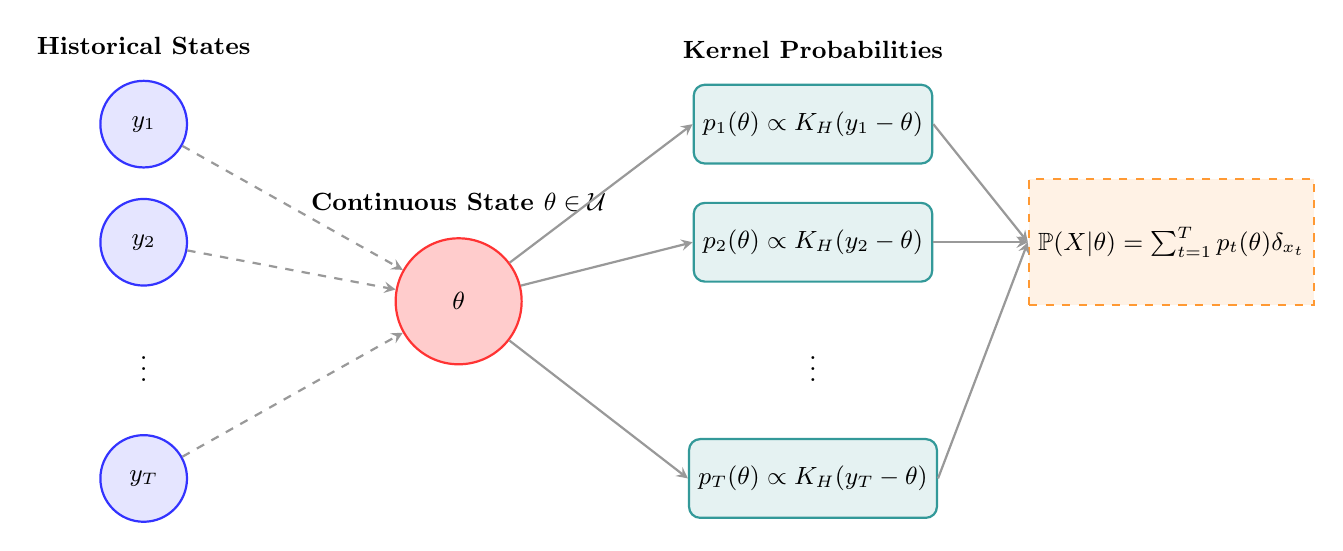
\begin{tikzpicture}[
    node distance=2cm,
    state/.style={circle, draw=blue!80, fill=blue!10, thick, minimum size=1.1cm, font=\small},
    kernel/.style={rectangle, draw=teal!80, fill=teal!10, rounded corners, thick, minimum height=1cm, font=\small},
    dist/.style={rectangle, draw=orange!80, fill=orange!10, dashed, thick, minimum width=3.4cm, minimum height=1.6cm, font=\small},
    arrow/.style={thick, ->, >=stealth, color=gray!80}
]

\node[state] (y1) at (0, 3) {$y_1$};
\node[state] (y2) at (0, 1.5) {$y_2$};
\node at (0, 0) {\vdots};
\node[state] (yT) at (0, -1.5) {$y_T$};

\node[above=0.2cm of y1, font=\bfseries\small] {Historical States};

\node[state, fill=red!20, draw=red!80, minimum size=1.6cm] (theta) at (4, 0.75) {$\theta$};
\node[above=0.2cm of theta, font=\bfseries\small] {Continuous State $\theta \in \mathcal{U}$};

\node[kernel] (k1) at (8.5, 3) {$p_1(\theta) \propto K_H(y_1 - \theta)$};
\node[kernel] (k2) at (8.5, 1.5) {$p_2(\theta) \propto K_H(y_2 - \theta)$};
\node at (8.5, 0) {\vdots};
\node[kernel] (kT) at (8.5, -1.5) {$p_T(\theta) \propto K_H(y_T - \theta)$};

\node[above=0.2cm of k1, font=\bfseries\small] {Kernel Probabilities};

\draw[arrow, dashed] (y1) -- (theta);
\draw[arrow, dashed] (y2) -- (theta);
\draw[arrow, dashed] (yT) -- (theta);

\draw[arrow] (theta) -- (k1.west);
\draw[arrow] (theta) -- (k2.west);
\draw[arrow] (theta) -- (kT.west);

\node[dist, right=1.2cm of k2] (cond_dist) {$\mathbb{P}(X | \theta) = \sum_{t=1}^T p_t(\theta) \delta_{x_t}$};
\draw[arrow] (k1.east) -- (cond_dist.west);
\draw[arrow] (k2.east) -- (cond_dist.west);
\draw[arrow] (kT.east) -- (cond_dist.west);

\end{tikzpicture}
}
\caption{Continuous market state mapping using multivariate Gaussian kernel weighting to construct conditional empirical return distributions from observable financial indicators}
\label{fig:schema1}
\end{figure}

\subsection{Semi-infinite programming formulation and theoretical properties}
Let $w = (w_1, \dots, w_N)^\top \in \mathbb{R}^N$ denote the portfolio weight vector. The portfolio loss under realized return vector $x_t$ is $-x_t^\top w$. We define the feasible portfolio set $W \subset \mathbb{R}^N$ under standard institutional long-only constraints with an individual weight cap $\bar{w} = 0.15$ and a target expected return constraint:
\begin{equation}
    W = \left\{ w \in \mathbb{R}^N : \sum_{i=1}^N w_i = 1, \quad 0 \le w_i \le \bar{w} \quad \forall i=1,\dots,N, \quad \hat{\mu}^\top w \ge \mu_{\text{target}} \right\}
\end{equation}
where $\hat{\mu} = \frac{1}{T} \sum_{t=1}^T x_t$ is the unconditional sample mean return vector, $\mu_{\text{target}}$ is the required expected return, and $\bar{w} = 0.15$ is the maximum allocation to any single asset.

\begin{proposition}[Feasibility of the capped portfolio set]
Let $S_{\bar w}=\{w \in \mathbb{R}^N : \mathbf{1}^\top w=1,\ 0\leq w_i\leq\bar w\}$. Then $S_{\bar w}\neq\emptyset$ if and only if $N\bar w\geq 1$. Conditional on this, let $\hat{\mu}_{(1)} \ge \dots \ge \hat{\mu}_{(N)}$ be the components of $\hat{\mu}$ sorted in descending order, and $\hat{\mu}_{[1]} \le \dots \le \hat{\mu}_{[N]}$ be sorted in ascending order. Define $q = \lfloor 1/\bar{w} \rfloor$ and the residual weight $r = 1 - q \bar{w}$. The maximum and minimum expected returns attainable in $S_{\bar w}$ are respectively $\mu_{\max} = \bar{w} \sum_{i=1}^q \hat{\mu}_{(i)} + (r > 0 ? r \hat{\mu}_{(q+1)} : 0)$ and $\mu_{\min} = \bar{w} \sum_{i=1}^q \hat{\mu}_{[i]} + (r > 0 ? r \hat{\mu}_{[q+1]} : 0)$, with the residual term omitted when $r=0$. The attainable expected-return set is $[\mu_{\min}, \mu_{\max}]$. Then $W\neq\emptyset$ if and only if $\mu_{\mathrm{target}}\leq\mu_{\max}$. Moreover, there exists $w\in S_{\bar w}$ satisfying $\hat\mu^\top w>\mu_{\mathrm{target}}$ if and only if $\mu_{\mathrm{target}}<\mu_{\max}$.
\end{proposition}

\begin{proof}
If $N\bar{w} < 1$, then $\sum_{i=1}^N w_i \le N\bar{w} < 1$, so no fully invested portfolio exists. When $N\bar{w} \ge 1$, the continuous knapsack problem $\max\{\hat{\mu}^\top w : \mathbf{1}^\top w = 1, 0 \le w_i \le \bar{w}\}$ is solved greedily by setting $w_{(i)} = \bar{w}$ for the $q$ assets with largest mean returns, and assigning the residual weight $r = 1 - q\bar{w}$ to the $(q+1)$-th asset, yielding the upper bound $\mu_{\max}$. The set $W$ is the intersection of closed half-spaces and the compact unit simplex, hence compact and convex.
\end{proof}

Following \citet{rockafellar2000optimization}, the conditional CVaR evaluated at state $\theta$ at confidence level $\alpha = 1 - \tau$ (with $\tau = 0.05$) is:
\begin{equation}
    \Phi_\tau(w, \theta) = \min_{z \in \mathbb{R}} \left\{ z + \frac{1}{\tau} \sum_{t=1}^T p_t(\theta) [-x_t^\top w - z]_+ \right\}
\end{equation}
where $z \in \mathbb{R}$ represents the conditional Value-at-Risk (VaR) at level $\alpha = 1 - \tau$, and $[u]_+ = \max(0, u)$. The optimal VaR minimizer satisfies $z^*(\theta) \in \operatorname{VaR}_{1-\tau}(\ell(w) \mid \theta)$. Although $z^*(\theta)$ may be a non-singleton interval for discrete empirical distributions, the minimum value $\Phi_\tau(w, \theta)$ is uniquely defined.

The continuous-state robust portfolio optimization problem seeks an allocation $w \in W$ that minimizes the worst-case conditional CVaR across all market states in $\mathcal{U}$:
\begin{equation}
    v^\star = \min_{w \in W} \sup_{\theta \in \mathcal{U}} \Phi_\tau(w, \theta)
\end{equation}
Introducing an auxiliary epigraph scalar $\eta \in \mathbb{R}$ representing the robust risk level, the problem is formulated as the following convex Semi-Infinite Program (SIP):
\begin{align}
    \min_{w \in \mathbb{R}^N, \eta \in \mathbb{R}} \quad & \eta \\
    \text{s.t.} \quad & \Phi_\tau(w, \theta) \le \eta \quad \forall \theta \in \mathcal{U} \\
    & \sum_{i=1}^N w_i = 1 \\
    & 0 \le w_i \le \bar{w} \quad \forall i=1,\dots,N \\
    & \hat{\mu}^\top w \ge \mu_{\text{target}}
\end{align}

\begin{proposition}[Compactness, continuity, and convexity]
Assume that $H \succ 0$, $N\bar{w} \ge 1$, and $\mu_{\text{target}} \le \mu_{\max}$. Then:
\begin{enumerate}
    \item The feasible portfolio set $W$ and the market state space $\mathcal{U}$ are non-empty, compact subsets of $\mathbb{R}^N$ and $\mathbb{R}^2$, respectively.
    \item For every $t = 1, \dots, T$, the kernel weight function $\theta \mapsto p_t(\theta)$ is infinitely differentiable and strictly positive on $\mathcal{U}$.
    \item The conditional CVaR function $(w, \theta) \mapsto \Phi_\tau(w, \theta)$ is jointly continuous on $W \times \mathcal{U}$.
    \item For every fixed $\theta \in \mathcal{U}$, the function $w \mapsto \Phi_\tau(w, \theta)$ is real-valued and convex on $W$.
\end{enumerate}
\end{proposition}

\begin{proof}
Item 1 follows from Proposition 1 and the closed bounding box construction of $\mathcal{U}$. For Item 2, the Gaussian kernel $K_H(u)$ is smooth and strictly positive on $\mathbb{R}^2$. The normalization denominator $\sum_{s=1}^T K_H(y_{s-1} - \theta)$ is strictly positive on compact $\mathcal{U}$. Thus $p_t(\theta)$ is a ratio of smooth, positive functions with a non-vanishing denominator, making it smooth and strictly positive. For Item 3, for each fixed $t$, the loss function $(w, z) \mapsto [-x_t^\top w - z]_+$ is jointly continuous and convex. Because $p_t(\theta)$ is continuous, the function $F(w, z, \theta) = z + \frac{1}{\tau} \sum_{t=1}^T p_t(\theta) [-x_t^\top w - z]_+$ is jointly continuous on $\mathbb{R}^N \times \mathbb{R} \times \mathcal{U}$. The partial minimization over $z$ is restricted to a compact interval $[-M_L, M_L]$, where $M_L = \max_{w \in W, t} |x_t^\top w| < \infty$. Since a weighted empirical VaR minimizer can always be selected between the minimum and maximum portfolio losses, we restrict $z$ to this compact set. By Berge's Maximum Theorem, the marginal function $\Phi_\tau(w, \theta) = \min_z F(w, z, \theta)$ is continuous on $W \times \mathcal{U}$. For Item 4, for fixed $\theta$, $\Phi_\tau(\cdot, \theta)$ is the partial minimization over $z$ of the jointly convex function $(w, z) \mapsto F(w, z, \theta)$, which preserves convexity in $w$.
\end{proof}

\begin{theorem}[Existence of optimal robust allocation]
Under the assumptions of Proposition 2, the robust objective function $G(w) = \sup_{\theta \in \mathcal{U}} \Phi_\tau(w, \theta)$ is continuous and convex on $W$. Furthermore, the supremum is attained for every $w \in W$, and the continuous-state robust portfolio optimization problem admits an optimal solution $w^* \in W$.
\end{theorem}

\begin{proof}
Because $\mathcal{U}$ is compact and $\Phi_\tau(w, \cdot)$ is continuous on $\mathcal{U}$ for every $w \in W$, the Extreme Value Theorem guarantees that the supremum is achieved at some $\theta^*(w) \in \mathcal{U}$, so $G(w) = \max_{\theta \in \mathcal{U}} \Phi_\tau(w, \theta)$. As the pointwise maximum of a family of convex functions $\{w \mapsto \Phi_\tau(w, \theta)\}_{\theta \in \mathcal{U}}$, $G(w)$ is convex on $W$. Joint continuity of $\Phi_\tau(w, \theta)$ on compact $W \times \mathcal{U}$ implies by Berge's Maximum Theorem that $G(w)$ is continuous on $W$. Finally, minimizing the continuous function $G(w)$ over the non-empty compact set $W$ guarantees the existence of an optimal solution $w^* \in W$ by the Weierstrass Theorem.
\end{proof}

\section{The adaptive semi-infinite exchange algorithm}
Direct discretization of the continuous state space $\mathcal{U}$ over a fine Cartesian grid $\widehat{\mathcal{U}} = \{\theta_1, \dots, \theta_K\}$ yields a large-scale linear program with $K \times T$ auxiliary variables and constraints. For realistic rolling backtests requiring hundreds of sequential optimizations, dense grid solvers suffer from excessive memory footprints and slow convergence. We design an adaptive exchange algorithm that iteratively generates only the binding stress states.

\subsection{Master problem and separation oracle}
At iteration $k \ge 1$, the master problem optimizes portfolio weights $w$ and the robust risk level $\eta$ subject to a finite active subset of market states $\mathcal{U}_k = \{\theta^{(1)}, \dots, \theta^{(m_k)}\} \subset \mathcal{U}$. For each active state $\theta^{(j)} \in \mathcal{U}_k$, we introduce a state-specific VaR variable $z_{\theta^{(j)}} \in \mathbb{R}$ and scenario excess loss variables $u_{t, \theta^{(j)}} \ge 0$. The master problem is the following finite Linear Program (LP):
\begin{align}
    \text{LB}_k = \min_{w, \eta, \{z_\theta\}, \{u_{t,\theta}\}} \quad & \eta \\
    \text{s.t.} \quad & z_\theta + \frac{1}{\tau} \sum_{t=1}^{T} p_t(\theta) u_{t,\theta} \le \eta \quad \forall \theta \in \mathcal{U}_k \\
    & u_{t,\theta} \ge -x_t^\top w - z_\theta \quad \forall t=1,\dots,T, \forall \theta \in \mathcal{U}_k \\
    & u_{t,\theta} \ge 0 \quad \forall t=1,\dots,T, \forall \theta \in \mathcal{U}_k \\
    & \sum_{i=1}^N w_i = 1, \quad 0 \le w_i \le \bar{w} \quad \forall i=1,\dots,N \\
    & \hat{\mu}^\top w \ge \mu_{\text{target}}
\end{align}
Solving the master LP yields a candidate allocation $w_k$ and a lower bound $\text{LB}_k$ on the true optimal value $v^\star$, because $\mathcal{U}_k \subset \mathcal{U}$ represents a relaxed constraint set.

Given $w_k$, the separation oracle searches for the most adverse state that maximizes conditional CVaR. In our empirical implementation, the separation step searches a candidate discretization $\widehat{\mathcal{U}} \subset \mathcal{U}$ ($21 \times 21 = 441$ states):
\begin{equation}
    \theta^* = \arg\max_{\theta \in \widehat{\mathcal{U}}} \Phi_\tau(w_k, \theta), \qquad \widehat{G}_k = \Phi_\tau(w_k, \theta^*)
\end{equation}

For computational tractability, we replace the continuous domain $\mathcal{U}$ with a finite candidate grid $\widehat{\mathcal{U}}$, resulting in the grid-restricted robust approximation:
\begin{equation}
    \widehat{v}^\star = \min_{w \in W} \max_{\theta \in \widehat{\mathcal{U}}} \Phi_\tau(w, \theta)
\end{equation}
Every numerical ``optimal'', ``worst-case'', or ``binding'' claim regarding our adaptive exchange algorithm refers to $\widehat{v}^\star$ over $\widehat{\mathcal{U}}$, not the continuous domain $\mathcal{U}$.


The conditional CVaR evaluation $\Phi_	au(w_k, 	heta)$ is computed in $O(T \log T + KT)$ time across the $K$ grid states by sorting portfolio losses once $\ell_t = -x_t^\top w_k$ in ascending order $\ell_{(1)} \le \dots \le \ell_{(T)}$ and identifying the index $j$ where the cumulative kernel weight reaches $1 - \tau = 0.95$:
\begin{equation}
    j^* = \min \left\{ j \in \{1,\dots,T\} : \sum_{t=1}^j p_{(t)}(\theta) \ge 1 - \tau \right\}
\end{equation}
The optimal conditional VaR is $z^*(\theta) = \ell_{(j^*)}$, and the conditional CVaR is evaluated directly from the tail excess losses. The overall adaptive exchange algorithm is depicted in Figure \ref{fig:schema2}.

\begin{figure}[htbp]
\centering
\resizebox{0.88\textwidth}{!}{
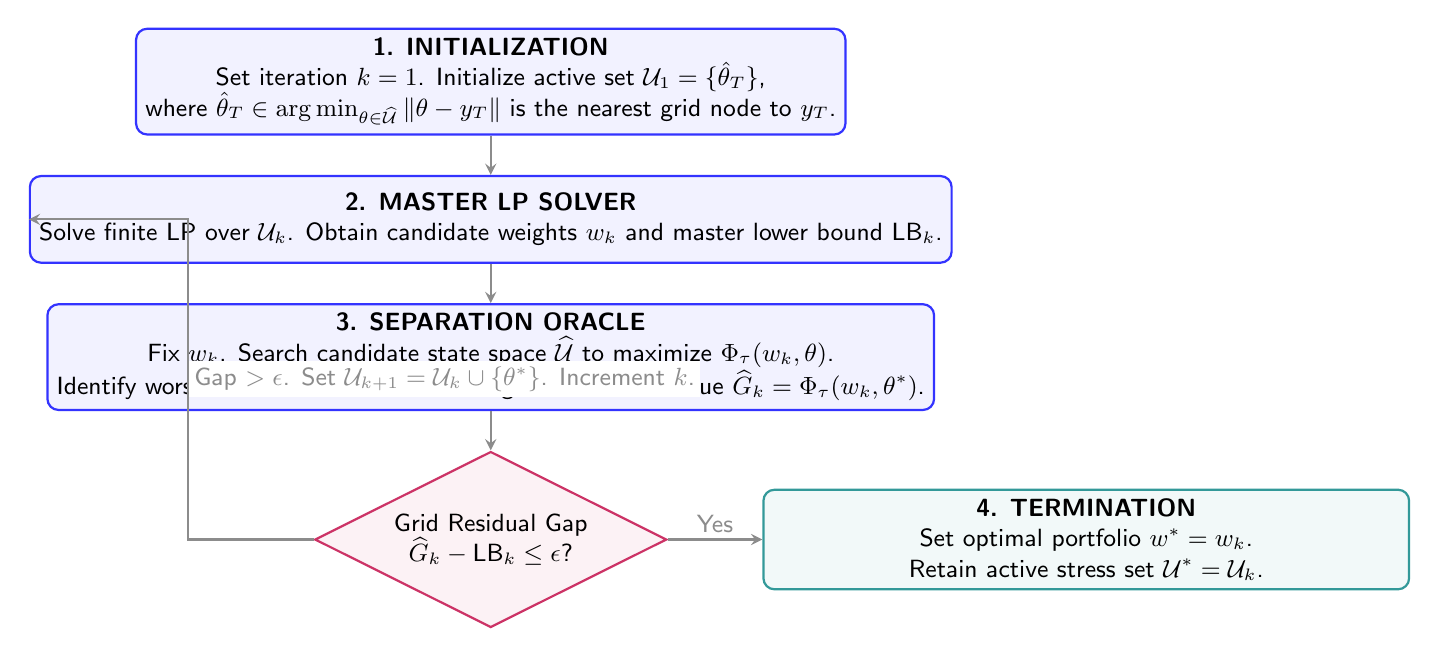
\begin{tikzpicture}[
    node distance=1.4cm, 
    every node/.style={fill=white, font=\sffamily\small}, 
    box/.style={draw=blue!80, fill=blue!5, rectangle, rounded corners, thick, minimum width=8.2cm, minimum height=1.1cm, align=center},
    arrow/.style={thick, ->, >=stealth, color=gray!90}
]
\node (step1) [box] {\textbf{1. INITIALIZATION}\\Set iteration $k=1$. Initialize active set $\mathcal{U}_1 = \{\hat\theta_T\}$,\\where $\hat\theta_T \in \arg\min_{\theta \in \widehat{\mathcal{U}}} \|\theta - y_T\|$ is the nearest grid node to $y_T$.};
\node (step2) [box, below=0.5cm of step1] {\textbf{2. MASTER LP SOLVER}\\Solve finite LP over $\mathcal{U}_k$. Obtain candidate weights $w_k$ and master lower bound $\text{LB}_k$.};
\node (step3) [box, below=0.5cm of step2] {\textbf{3. SEPARATION ORACLE}\\Fix $w_k$. Search candidate state space $\widehat{\mathcal{U}}$ to maximize $\Phi_\tau(w_k, \theta)$.\\Identify worst-case state $\theta^*$ and evaluate grid worst-case value $\widehat{G}_k = \Phi_\tau(w_k, \theta^*)$.};
\node (check) [draw=purple!80, fill=purple!5, diamond, aspect=2, thick, below=0.5cm of step3, align=center] {Grid Residual Gap\\$\widehat{G}_k - \text{LB}_k \le \epsilon$?};
\node (step6) [box, draw=teal!80, fill=teal!5, right=1.2cm of check] {\textbf{4. TERMINATION}\\Set optimal portfolio $w^* = w_k$.\\Retain active stress set $\mathcal{U}^* = \mathcal{U}_k$.};

\draw [arrow] (step1) -- (step2);
\draw [arrow] (step2) -- (step3);
\draw [arrow] (step3) -- (check);
\draw [arrow] (check.west) -- ++(-1.6,0) |- node[pos=0.25, right, fill=white, inner sep=2pt] {Gap $> \epsilon$. Set $\mathcal{U}_{k+1} = \mathcal{U}_k \cup \{\theta^*\}$. Increment $k$.} (step2.west);
\draw [arrow] (check.east) -- node[above, fill=white, inner sep=2pt] {Yes} (step6.west);

\end{tikzpicture}
}
\caption{The Adaptive Semi-Infinite Programming (SIP) exchange algorithm. The master linear program and the separation oracle interact iteratively to isolate the binding stress states that define the robust allocation}
\label{fig:schema2}
\end{figure}

\subsection{Convergence analysis with exact and inexact oracles}
We establish theoretical convergence guarantees for both exact global separation and grid-restricted separation.

\begin{proposition}[Convergence under exact separation]
Assume that each master problem is solved to exact LP optimality and the separation oracle identifies the worst-case state $\theta^* = \arg\max_{\theta \in \mathcal{U}} \Phi_\tau(w_k, \theta)$ with exact value $G(w_k) = \Phi_\tau(w_k, \theta^*)$. Then:
\begin{enumerate}
    \item The master lower bounds form a non-decreasing sequence: $\text{LB}_1 \le \text{LB}_2 \le \dots \le v^\star$.
    \item The oracle values satisfy $G(w_k) \ge v^\star$ for all $k \ge 1$.
    \item For any convergence tolerance $\epsilon > 0$, the exchange algorithm terminates in a finite number of iterations with an $\epsilon$-optimal portfolio $w_k \in W$ satisfying:
    \begin{equation}
        0 \le G(w_k) - v^\star \le \epsilon, \qquad \sup_{\theta \in \mathcal{U}} \bigl[\Phi_\tau(w_k, \theta) - \text{LB}_k\bigr] \le \epsilon
    \end{equation}
\end{enumerate}
\end{proposition}

\begin{proof}
Because $\mathcal{U}_k \subset \mathcal{U}_{k+1} \subset \mathcal{U}$, the feasible region of the master LP shrinks monotonically, implying $\text{LB}_k \le \text{LB}_{k+1} \le v^\star$. For Item 2, $G(w_k) = \sup_{\theta \in \mathcal{U}} \Phi_\tau(w_k, \theta) \ge \min_{w \in W} \sup_{\theta \in \mathcal{U}} \Phi_\tau(w, \theta) = v^\star$.

For Item 3, upon termination with $G(w_k) - \text{LB}_k \le \epsilon$, we have $0 \le G(w_k) - v^\star \le G(w_k) - \text{LB}_k \le \epsilon$, and the portfolio $w_k$ satisfies all finite constraints in $W$ while the epigraph pair $(w_k, \text{LB}_k)$ is $\epsilon$-feasible for the continuous constraint set.

To establish finite termination, suppose for contradiction that the algorithm does not terminate. Then it generates an infinite sequence of states $\{\theta_k\}_{k=1}^\infty \subset \mathcal{U}$ such that $\Phi_\tau(w_k, \theta_k) - \text{LB}_k > \epsilon$ for all $k$. For any $j < k$, the constraint for $\theta_j$ was included in master problem $k$, so $\Phi_\tau(w_k, \theta_j) \le \text{LB}_k$. Thus $\Phi_\tau(w_k, \theta_k) - \Phi_\tau(w_k, \theta_j) > \epsilon$. Since $\Phi_\tau$ is continuous on the compact set $W\times \mathcal{U}$, it is uniformly continuous. Hence, for every $\varepsilon>0$, there exists $\delta_\varepsilon>0$ such that $\|\theta-\theta'\|<\delta_\varepsilon \implies |\Phi_\tau(w,\theta)-\Phi_\tau(w,\theta')|<\varepsilon$ uniformly for all $w\in W$. Therefore, $\|\theta_k - \theta_j\| \ge \delta_\epsilon$ for all $j < k$. A compact metric space is totally bounded and therefore cannot contain an infinite $\delta_\epsilon$-separated sequence, which contradicts the compactness of $\mathcal{U}$ \citep{hettich1993semi, lopez2007semi}. This exact-oracle convergence is a classical consequence of standard SIP exchange methods. This exact-oracle convergence is a classical consequence of standard SIP exchange methods.
\end{proof}

\begin{remark}[Monotonicity of bounds]
While the master lower bounds $\text{LB}_k$ are guaranteed to be monotonically non-decreasing, the separation oracle worst-case values $\widehat{G}(w_k)$ are not guaranteed to decrease monotonically at every iteration because the portfolio $w_k$ changes. However, the best incumbent worst-case value $\overline{G}_k = \min_{1 \le j \le k} \widehat{G}(w_j)$ is monotonically non-increasing by construction.
\end{remark}

\begin{remark}[Grid-restricted separation]
When the separation oracle is evaluated over a finite candidate grid $\widehat{\mathcal{U}} \subset \mathcal{U}$, it computes
\begin{equation}
\widehat{G}(w) = \max_{\theta \in \widehat{\mathcal{U}}} \Phi_\tau(w, \theta) \le \sup_{\theta \in \mathcal{U}} \Phi_\tau(w, \theta).
\end{equation}
Since $\Phi_\tau$ is continuous on the compact set $W \times \mathcal{U}$, it is uniformly continuous. Therefore, the discrepancy between the continuous and grid-restricted objectives tends to zero as the grid dispersion radius tends to zero. A quantitative $L_\Phi\rho$ bound would require an explicitly validated uniform Lipschitz constant. We do not compute such a constant in the empirical analysis and instead assess discretization sensitivity through grid refinement. To ensure the algorithm operates strictly over $\widehat{\mathcal{U}}$, the active subset $U_1$ is initialized with the nearest grid node to the most recent observation $y_T$.


The dispersion radius $\rho$ alone is a geometric grid statistic, not a continuous-optimality certificate. However, under standard assumptions, a conservative window-specific Lipschitz constant $L_\Phi$ for the conditional CVaR would provide the error bound:
\begin{equation}
0 \le \sup_{\theta \in \mathcal{U}} \Phi_\tau(w, \theta) - \max_{\theta \in \widehat{\mathcal{U}}} \Phi_\tau(w, \theta) \le L_\Phi \rho.
\end{equation}
Since we do not explicitly compute $L_\Phi$, we rely on grid-refinement sensitivity to validate the approximation.



The dispersion radius $\rho$ alone is a geometric grid statistic, not a continuous-optimality certificate. However, under standard assumptions, a conservative window-specific Lipschitz constant $L_\Phi$ for the conditional CVaR would provide the error bound:
\begin{equation}
0 \le \sup_{\theta \in \mathcal{U}} \Phi_\tau(w, \theta) - \max_{\theta \in \widehat{\mathcal{U}}} \Phi_\tau(w, \theta) \le L_\Phi \rho.
\end{equation}
Since we do not explicitly compute $L_\Phi$, we rely on grid-refinement sensitivity to validate the approximation.

\end{remark}

\section{Empirical framework and multi-decade results}
We evaluate the out-of-sample performance, turnover efficiency, downside capital preservation, and computational scalability of the continuous-state robust portfolio framework.

\subsection{Data and institutional backtesting protocol}
The empirical universe comprises the Kenneth French 30 Industry Portfolios (value-weighted daily returns), providing broad industry-level coverage of the US equity market. Daily asset returns are aligned with:
\begin{itemize}
    \item \textbf{CBOE VIX}: Daily closing prices of the CBOE Volatility Index.
    \item \textbf{Broad Market Drawdown}: Calculated daily from the equal-weighted 30-industry composite over trailing 63-day lookback windows ($D_t \in [0, 1]$).
\end{itemize}
The aligned daily dataset spans from January 1990 to 17 June 2026, comprising 9,186 daily observations.

\begin{figure}[htbp]
\centering
\resizebox{0.92\textwidth}{!}{
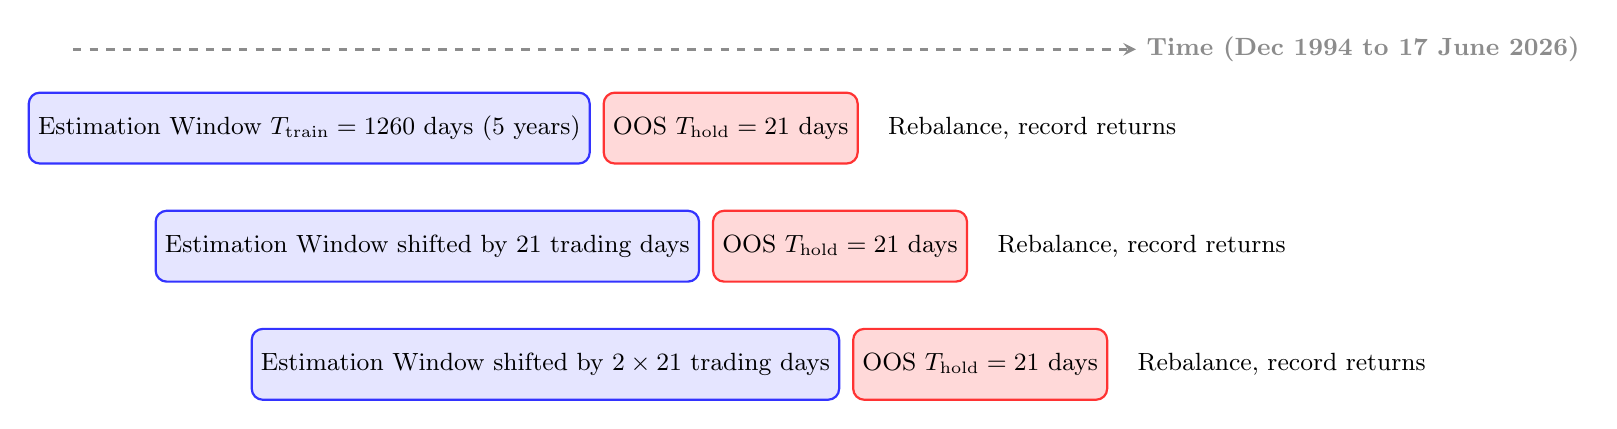
\begin{tikzpicture}[
    node distance=1cm,
    timeline/.style={draw=blue!80, fill=blue!10, thick, rounded corners, minimum height=0.9cm, font=\small},
    oos/.style={draw=red!80, fill=red!15, thick, rounded corners, minimum height=0.9cm, font=\small},
    arrow/.style={thick, ->, >=stealth, color=gray!90}
]

\node[timeline, minimum width=6cm] (train1) at (0, 2) {Estimation Window $T_{\text{train}} = 1260$ days (5 years)};
\node[oos, minimum width=1.8cm, right=0.15cm of train1] (test1) {OOS $T_{\text{hold}} = 21$ days};
\node[right=0.25cm of test1, font=\small] {Rebalance, record returns};

\node[timeline, minimum width=6cm] (train2) at (1.5, 0.5) {Estimation Window shifted by 21 trading days};
\node[oos, minimum width=1.8cm, right=0.15cm of train2] (test2) {OOS $T_{\text{hold}} = 21$ days};
\node[right=0.25cm of test2, font=\small] {Rebalance, record returns};

\node[timeline, minimum width=6cm] (train3) at (3.0, -1) {Estimation Window shifted by $2 \times 21$ trading days};
\node[oos, minimum width=1.8cm, right=0.15cm of train3] (test3) {OOS $T_{\text{hold}} = 21$ days};
\node[right=0.25cm of test3, font=\small] {Rebalance, record returns};

\draw[arrow, dashed, line width=1pt] (-3, 3) -- (10.5, 3) node[right, font=\bfseries\small] {Time (Dec 1994 to 17 June 2026)};

\end{tikzpicture}
}
\caption{The rolling-window backtesting protocol. Portfolios are re-optimized every 21 trading days using trailing 5-year estimation windows, and realized performance is evaluated out-of-sample over non-overlapping 21-day holding periods}
\label{fig:schema3}
\end{figure}

The backtest uses a rolling estimation window of $T_{\text{train}} = 1260$ trading days (approximately 5 years), as illustrated in Figure \ref{fig:schema3}. At each rebalancing date, the optimization models are estimated using only data available up to that point. The resulting allocations are held constant over the subsequent out-of-sample holding period of $T_{\text{hold}} = 21$ trading days. The backtest generates 377 consecutive 21-trading-day holding periods from 28 December 1994 to 17 June 2026.

To maintain strict benchmark fairness across all optimized models, the target expected return $\mu_{\text{target}}$ is dynamically set at each rebalancing date to the cross-sectional median of historical asset means: $\mu_{\text{target}} = \text{median}(\hat{\mu})$. The identical target return constraint $\hat{\mu}^\top w \ge \mu_{\text{target}}$ and weight cap $\bar{w} = 0.15$ are enforced on Robust SIP, Nominal CVaR, and Finite-Regime CVaR. In the computational implementation, $\mu_{\text{target}}$ is dynamically clamped to the attainable interval $[\mu_{\min}, \mu_{\max} - 10^{-6}]$ to guarantee strict feasibility. Over the 377 rolling out-of-sample evaluation windows, target return clamping occurred in exactly 0 periods, ensuring the original target specifications were strictly respected throughout the backtest.

We compare the continuous-state Robust SIP against four established benchmark strategies:
\begin{itemize}
    \item \textbf{1/N}: Naive equal-weighted portfolio $w_i = 1/N$.
    \item \textbf{Target-Constrained Minimum Variance (TC-MinVar)}: Minimizes portfolio variance $w^\top \widehat{\Sigma} w$ subject to $w \in W$, using the standard sample covariance matrix $\widehat{\Sigma}$. Solved via quadratic programming.
    \item \textbf{Nominal CVaR}: Minimizes unconditional historical CVaR at $95\%$ confidence level subject to $w \in W$, using uniform observation weights $1/T$.
    \item \textbf{Finite-Regime CVaR}: Minimizes the maximum CVaR across $K=4$ discrete regimes. Regimes are formed by independent median splits on log-VIX and trailing drawdown. Regime probabilities are uniform over the observations within each regime, and boundaries are recomputed in every rolling window.
\end{itemize}

To incorporate realistic market frictions, we compute holding-period portfolio turnover taking into account asset price drift over the holding period:
\begin{equation}
    \widetilde w_{i,t} = \frac{w_{i,t-1}(1+R_{i,t})}{\sum_{j=1}^N w_{j,t-1}(1+R_{j,t})}
\end{equation}
where $R_{i,t}$ is the cumulative simple/net return (and $1+R_{i,t}$ is the gross return) of asset $i$ over the 21-day holding period. Holding-period turnover and net return are defined as:
\begin{equation}
    \text{TO}_t = \frac{1}{2} \sum_{i=1}^N | w_{i,t} - \widetilde w_{i,t} |, \qquad r_{t}^{\text{net}} = r_{t}^{\text{gross}} - c \cdot \text{TO}_t
\end{equation}

\subsection{Long-term cumulative wealth and risk-adjusted performance}
Figure \ref{fig:wealth} displays the cumulative wealth trajectories of all five investment strategies net of 10 bps transaction costs on an initial \$1 investment. The naive $1/N$ portfolio delivers the highest final cumulative wealth of \$29.25, followed by the Finite-Regime CVaR portfolio (\$25.68), the continuous Robust SIP strategy (\$25.04), the Nominal CVaR portfolio (\$22.92), and the TC-MinVar portfolio (\$22.16).

\begin{figure}[H]
    \centering
    
\includegraphics[width=0.88\textwidth]{Fig1.pdf}
    \caption{Out-of-sample cumulative net wealth trajectory across investment strategies from 28 December 1994 to 17 June 2026, accounting for 10 bps transaction costs}
    \label{fig:wealth}
\end{figure}

\begin{table}[htbp]
\centering
\caption{Comprehensive out-of-sample performance summary (28 December 1994 to 17 June 2026, net of 10 bps transaction costs)}
\label{tab:performance}
\resizebox{\textwidth}{!}{
\begin{tabular}{lrrrrr}
\toprule
\textbf{Metric} & \textbf{1/N} & \textbf{TC-MinVar} & \textbf{Nominal CVaR} & \textbf{Finite-Regime} & \textbf{Robust SIP} \\
\midrule
Annualized Mean Return (\%) & 12.24 & 10.75 & 10.76 & 11.15 & 11.28 \\
Annualized Volatility (\%) & 17.00 & 12.31 & 12.23 & 12.38 & 13.95 \\
Sharpe Ratio & 0.720 & 0.873 & 0.880 & 0.901 & 0.809 \\
Sortino Ratio & 1.127 & 1.335 & 1.351 & 1.396 & 1.218 \\
Realized 95\% CVaR (Holding-Period, \%) & 11.16 & 8.18 & 8.00 & 7.92 & 9.31 \\
Realized 99\% CVaR (Holding-Period, \%) & 17.21 & 12.76 & 11.84 & 12.04 & 13.98 \\
Maximum Drawdown (\%) & -55.79 & -40.18 & -35.76 & -36.76 & -41.69 \\
CAGR (\%) & 11.34 & 10.45 & 10.48 & 10.88 & 10.79 \\
Calmar Ratio & 0.203 & 0.260 & 0.293 & 0.296 & 0.259 \\
Average Holding-Period Turnover (\%) & 1.69 & 7.02 & 8.23 & 8.78 & 9.48 \\
Annual TC Drag (bps) & 2.02 & 8.42 & 9.87 & 10.54 & 11.37 \\
Effective Number of Assets ($N_{\text{eff}}$) & 30.00 & 8.15 & 7.92 & 7.57 & 7.36 \\
Worst Holding-Period Return (\%) & -20.41 & -15.29 & -15.42 & -15.15 & -18.99 \\
Final Cumulative Wealth (\$) & 29.25 & 22.16 & 22.92 & 25.68 & 25.04 \\
\bottomrule
\end{tabular}
}
\end{table}

Table \ref{tab:performance} reports the complete 14-metric performance profile. Key findings include:
\begin{enumerate}
    \item \textbf{Return Generation}: Robust SIP achieves an annualized mean return of 11.28\%, outperforming Nominal CVaR (10.76\%) and TC-MinVar (10.75\%), and ranking second to naive $1/N$ (12.24\%) and Finite-Regime CVaR (11.15\%). The $1/N$ portfolio benefits from broad cross-sectional diversification and full exposure to the long-run equity market risk premium over the 31-year evaluation period.
    \item \textbf{Risk-Adjusted Ratios}: Finite-Regime CVaR achieves the highest Sharpe ratio (0.901), followed by Nominal CVaR (0.880) and TC-MinVar (0.873). Robust SIP records a Sharpe ratio of 0.809. The resulting allocations exhibit higher realized volatility and greater concentration. Determining whether this arises from return targeting, state conditioning, or sparse-boundary effects requires further decomposition.
    \item \textbf{Turnover and Concentration}: Robust SIP generates the highest average holding-period turnover (9.48\%) among optimized strategies, resulting from rolling-window re-estimation of the return--state relationship. The resulting transaction cost drag is 11.38 basis points per year. The effective number of assets ($N_{\text{eff}} = 7.36$) is the most concentrated, reflecting targeted sector exposures conditional on the state domain.
\end{enumerate}

\begin{figure}[H]
    \centering
    
\includegraphics[width=0.88\textwidth]{Fig2.pdf}
    \caption{Out-of-sample portfolio drawdowns over time across all strategies}
    \label{fig:drawdown}
\end{figure}

\subsection{Drawdown profiles and crisis-period performance}
Figure \ref{fig:drawdown} plots the time series of out-of-sample drawdowns. The naive $1/N$ strategy experiences severe capital destruction during major market dislocations, suffering a maximum peak-to-trough drawdown of $-55.79\%$ during the 2008 financial crisis. All optimized models restrict maximum drawdown relative to $1/N$: Nominal CVaR achieves the shallowest at $-35.76\%$, Finite-Regime CVaR reaches $-36.76\%$, and TC-MinVar reaches $-40.18\%$. Robust SIP records a maximum drawdown of $-41.70\%$, which is deeper than the unconditional CVaR benchmarks.

\begin{table}[htbp]
\centering
\caption{Realized out-of-sample returns and maximum drawdowns across historical crisis periods}
\label{tab:crisis}
\resizebox{0.88\textwidth}{!}{
\begin{tabular}{llrr}
\toprule
\textbf{Crisis Period} & \textbf{Strategy} & \textbf{Cumulative Return (\%)} & \textbf{Maximum Drawdown (\%)} \\
\midrule
\textbf{Dot-Com Crash} & 1/N & -4.75 & -24.41 \\
(Mar 2000 to Oct 2002) & TC-MinVar & +1.36 & -20.66 \\
& Nominal CVaR & +5.86 & -20.66 \\
& Finite-Regime & +17.26 & -20.33 \\
& \textbf{Robust SIP} & \textbf{+4.25} & \textbf{-24.95} \\
\midrule
\textbf{Global Financial Crisis} & 1/N & -53.56 & -55.79 \\
(Oct 2007 to Mar 2009) & TC-MinVar & -34.67 & -40.18 \\
& Nominal CVaR & -31.13 & -35.76 \\
& Finite-Regime & -30.91 & -36.76 \\
& \textbf{Robust SIP} & \textbf{-36.49} & \textbf{-41.69} \\
\midrule
\textbf{COVID-19 Shock} & 1/N & -20.18 & -20.64 \\
(Feb 2020 to Apr 2020) & TC-MinVar & -12.25 & -15.29 \\
& Nominal CVaR & -12.05 & -15.42 \\
& Finite-Regime & -11.67 & -15.15 \\
& \textbf{Robust SIP} & \textbf{-17.44} & \textbf{-18.99} \\
\midrule
\textbf{Inflation Tightening} & 1/N & -6.05 & -17.24 \\
(Jan 2022 to Dec 2022) & TC-MinVar & -6.47 & -18.12 \\
& Nominal CVaR & -4.83 & -17.92 \\
& Finite-Regime & -7.66 & -18.88 \\
& \textbf{Robust SIP} & \textbf{-8.59} & \textbf{-19.86} \\
\bottomrule
\end{tabular}
}
\end{table}

Table \ref{tab:crisis} presents the crisis-period analysis. During the Dot-Com crash, Finite-Regime CVaR achieved the highest cumulative return (+17.26\%), followed by Nominal CVaR (+5.86\%) and Robust SIP (+4.25\%), while $1/N$ suffered the most ($-4.75\%$). In the Global Financial Crisis, Nominal CVaR provided the best downside protection ($-31.13\%$ cumulative, $-35.76\%$ maximum drawdown), while Robust SIP experienced a deeper drawdown of $-41.69\%$. During the COVID-19 crash, all optimized models limited losses to the $-11\%$ to $-17\%$ range, with Robust SIP absorbing a larger loss ($-17.44\%$) than the unconditional benchmarks ($-12\%$). In the 2022 inflation-driven selloff, Nominal CVaR was most resilient ($-4.83\%$), while Robust SIP suffered a larger cumulative loss ($-8.59\%$). These results reveal that continuous-state conditioning does not uniformly improve crisis-period performance; rather, it reshapes the allocation profile in ways that can amplify exposure during acute market dislocations.

\begin{figure}[htbp]
    \centering
    \begin{minipage}{0.48\textwidth}
        \centering
        
\includegraphics[width=\textwidth]{Fig3.pdf}
        \caption{Robust SIP asset allocations over time across the 30 industry portfolios (max 15\% cap)}
        \label{fig:weights_rob}
    \end{minipage}
    \hfill
    \begin{minipage}{0.48\textwidth}
        \centering
        
\includegraphics[width=\textwidth]{Fig4.pdf}
        \caption{TC-MinVar asset allocations over time across the 30 industry portfolios (max 15\% cap)}
        \label{fig:weights_mv}
    \end{minipage}
\end{figure}

Figures \ref{fig:weights_rob} and \ref{fig:weights_mv} compare the dynamic allocation weights of Robust SIP and TC-MinVar. Robust SIP maintains allocations across 7 to 10 active industry sectors ($N_{\text{eff}} = 7.36$), reallocating capital across cyclical and defensive sectors as historical window dynamics evolve. Conversely, the TC-MinVar portfolio remains concentrated in low-beta industries ($N_{\text{eff}} = 8.15$), and exhibits lower realized volatility and different sector exposures.

\begin{figure}[H]
    \centering
    
\includegraphics[width=0.88\textwidth]{Fig5.pdf}
    \caption{Distribution of holding-period portfolio turnover for all dynamic investment strategies}
    \label{fig:turnover}
\end{figure}

Figure \ref{fig:turnover} confirms that the turnover distribution for Robust SIP has a mean near 9.5\%, reflecting the active rebalancing induced by continuous state conditioning. TC-MinVar exhibits lower mean turnover (7.0\%), while $1/N$ has the lowest (1.7\%) due to its static equal-weight target.


\begin{figure}[H]
    \centering
    
\includegraphics[width=0.88\textwidth]{Fig6.pdf}
    \caption{Cumulative transaction cost impact over the out-of-sample period, assuming 10 bps proportional friction}
    \label{fig:cumulative_tc}
\end{figure}


\begin{table}[htbp]
\centering
\caption{Transaction cost sensitivity: out-of-sample performance under alternative cost levels}
\label{tab:tc_sensitivity}
\resizebox{0.92\textwidth}{!}{
\begin{tabular}{lrrrrr}
\toprule
\textbf{Strategy} & \textbf{TC = 0 bps} & \textbf{TC = 5 bps} & \textbf{TC = 10 bps} & \textbf{TC = 20 bps} & \textbf{TC = 50 bps} \\
\midrule
\textbf{Annualized Sharpe Ratio} & & & & & \\
1/N & 0.721 & 0.720 & 0.720 & 0.719 & 0.715 \\
TC-MinVar & 0.880 & 0.876 & 0.873 & 0.866 & 0.846 \\
Nominal CVaR & 0.888 & 0.884 & 0.880 & 0.872 & 0.848 \\
Finite-Regime & 0.909 & 0.905 & 0.901 & 0.892 & 0.867 \\
\textbf{Robust SIP} & \textbf{0.817} & \textbf{0.813} & \textbf{0.809} & \textbf{0.801} & \textbf{0.777} \\
\midrule
\textbf{Final Cumulative Wealth (\$)} & & & & & \\
1/N & 29.43 & 29.34 & 29.25 & 29.06 & 28.52 \\
TC-MinVar & 22.74 & 22.45 & 22.16 & 21.59 & 19.97 \\
Nominal CVaR & 23.63 & 23.27 & 22.92 & 22.22 & 20.26 \\
Finite-Regime & 26.53 & 26.10 & 25.68 & 24.85 & 22.52 \\
\textbf{Robust SIP} & \textbf{25.94} & \textbf{25.49} & \textbf{25.04} & \textbf{24.17} & \textbf{21.74} \\
\bottomrule
\end{tabular}
}
\end{table}

Table \ref{tab:tc_sensitivity} examines transaction cost sensitivity across 0, 5, 10, 20, and 50 bps. Finite-Regime CVaR dominates in risk-adjusted terms across all cost levels, maintaining a Sharpe ratio above 0.867 even at 50 bps. Robust SIP remains competitive in absolute wealth generation: at 50 bps, its final wealth of \$21.74 exceeds Nominal CVaR (\$20.26) and TC-MinVar (\$19.97), though it trails Finite-Regime (\$22.52). The $1/N$ portfolio is least sensitive to transaction costs due to its minimal turnover, retaining \$28.52 at 50 bps.

\subsection{Computational scalability, state density, and bootstrap inference}
Figure \ref{fig:active_states} illustrates the number of active stress states retained by the master problem across all 377 rolling backtest windows. Across the entire 31-year backtest, the algorithm consistently converges while retaining between 1 and 9 active market states (average 3.66) out of the 441 candidate states in $\widehat{\mathcal{U}}$. Because the algorithm adds exactly one state per iteration, the number of active states coincides with the number of exchange iterations (average 3.66 iterations).

\begin{figure}[H]
    \centering
    
\includegraphics[width=0.88\textwidth]{Fig7.pdf}
    \caption{Number of active stress states generated by the adaptive exchange algorithm across rolling backtest windows}
    \label{fig:active_states}
\end{figure}

\begin{figure}[H]
    \centering
    
\includegraphics[width=0.88\textwidth]{Fig8.pdf}
    \caption{Convergence of the Master LP Lower Bound ($\text{LB}_k$, royal blue line) and the Grid Separation Worst-Case Value ($\widehat{G}_k$, crimson red line) across adaptive exchange iterations.}
    \label{fig:bounds}
\end{figure}

Figure \ref{fig:bounds} tracks the convergence of the Master LP Lower Bound ($\text{LB}_k$) and the Grid Separation Worst-Case Value ($\widehat{G}_k$). The shaded green area denotes the grid-restricted exchange gap ($\widehat{G}_k - \text{LB}_k$). Starting from an initial gap at iteration $k=1$, the oracle worst-case value fluctuates as the portfolio changes, while the master lower bound increases monotonically and the residual gap eventually closes. After 3 exchange iterations, the grid-restricted residual gap falls below $10^{-4}$, confirming numerical convergence to the finite robust problem over the $21\times 21$ candidate grid.

\begin{table}[htbp]
\centering
\caption{Computational benchmark: adaptive exchange algorithm vs. dense grid approximation}
\label{tab:computational}
\resizebox{1.0\textwidth}{!}{
\begin{tabular}{llrlr}
\toprule
\textbf{Method} & \textbf{Status} & \textbf{Constraints} & \textbf{Runtime} & \textbf{Reported value} \\
\midrule
Adaptive SIP $21\times 21$ & OPTIMAL / tolerance reached & 5 & 3.45 s & final grid worst-case CVaR $\approx$ 3.3585\% \\
Dense $21\times 21$ & OPTIMAL & 441 & 71.43 s & optimum $\approx$ 3.3578\% \\
Dense $41\times 41$ & TIME\_LIMIT / no primal solution & 1681 & 632.25 s & --- \\
\bottomrule
\end{tabular}
}
\end{table}

\begin{table}[htbp]
\centering
\caption{Geometric grid diagnostic for the $21 \times 21$ grid}
\label{tab:grid_bounds}
\begin{tabular}{lc}
\toprule
\textbf{Diagnostic Metric} & \textbf{Value} \\
\midrule
Geometric grid radius $\rho$ (unit-dependent) & 0.032 \\
\bottomrule
\end{tabular}
\end{table}

\begin{table}[htbp]
\centering
\caption{Distribution of the window-level mean ESS across active stress states}
\label{tab:ess_diagnostics}
\begin{tabular}{lc}
\toprule
\textbf{Diagnostic Metric} & \textbf{Value} \\
\midrule
Minimum window-level mean ESS & 2.18 \\
5th Percentile window-level mean ESS & 16.98 \\
Median window-level mean ESS & 72.75 \\
Mean window-level mean ESS & 83.02 \\
Maximum window-level mean ESS & 264.36 \\
Mean window-level effective tail count ($\tau \times \overline{\mathrm{ESS}}$) & 4.15 \\
\bottomrule
\end{tabular}
\end{table}

Table \ref{tab:computational} provides a quantitative comparison between the adaptive exchange algorithm and dense Cartesian grid solutions. Using the representative-window benchmark, the adaptive algorithm with 5 active states solves in 3.45 seconds, compared to 71.43 seconds for the $21 \times 21$ grid (441 states), achieving approximately a $20.7\times$ speedup on the representative benchmark window relative to the $21 \times 21$ grid. The dense $41 \times 41$ formulation did not return a primal solution within the 600-second solver limit; therefore, no objective value or allocation distance is reported.

Several diagnostics in Tables \ref{tab:computational} and \ref{tab:ess_diagnostics} warrant careful interpretation:
\begin{enumerate}
    \item \textbf{Representative-Window $\ell_1$ Weight Discrepancy}: On the representative window, the $\ell_1$ distance between the adaptive $21 \times 21$ exchange solution and the dense $21 \times 21$ grid solution is $\|w_{\mathrm{adaptive}}-w_{\mathrm{dense21}}\|_1 \approx 0.00156$. The difference between the adaptive final grid worst-case value and the dense-grid optimum is approximately $7.6\times10^{-6}$, below the exchange tolerance of $10^{-4}$.
    \item \textbf{Tail Effective Sample Size}: The minimum, across rolling windows, of the within-window mean ESS over active states is 2.18, indicating that some windows contain collectively low-support active stress states. State-level exports would be required to identify the minimum individual active-state ESS and determine whether it occurs at the boundary of the state domain.
\end{enumerate}


\begin{figure}[htbp]
    \centering
    
\includegraphics[width=0.88\textwidth]{Fig9.pdf}
    \caption{Evolution of the average Effective Sample Size (ESS) for active stress states across the 377 rolling backtest windows}
    \label{fig:ess_history}
\end{figure}


\begin{figure}[htbp]
    \centering
    \begin{minipage}{0.48\textwidth}
        \centering
        
\includegraphics[width=\textwidth]{Fig10.pdf}
        \caption{In-sample risk-return efficient frontiers (15\% weight cap)}
        \label{fig:frontier}
    \end{minipage}
    \hfill
    \begin{minipage}{0.48\textwidth}
        \centering
        
\includegraphics[width=\textwidth]{Fig11.pdf}
        \caption{State density and active stress states. The grid nodes are generated in log-VIX coordinates, and the displayed density includes the Jacobian of the exponential transformation}
        \label{fig:kernel}
    \end{minipage}
\end{figure}

Figure \ref{fig:frontier} contextualizes the in-sample decision environment. The continuous-state robust efficient frontier forms an outer envelope of worst-case risk across all states in $\mathcal{U}$, positioned to the right of the unconditional nominal CVaR frontier and the classical Markowitz mean-variance frontier. Individual industry portfolios exhibit substantial dispersion in both expected return and downside tail risk, with defensive sectors displaying lower tail risk compared to high-beta sectors.

Figure \ref{fig:kernel} visualizes the continuous market-state space $\mathcal{U} \subset \mathbb{R}^2$ alongside the bivariate kernel density estimate $f(\text{log-VIX}, \text{Drawdown})$. Historical market states concentrate in a low-volatility, low-drawdown core regime (VIX between 10 and 20, Drawdown below 10\%). However, the continuous domain extends outward into severe tail regions, encompassing major historical dislocations such as the 1998 LTCM collapse (VIX 45.74, Drawdown 19.3\%), the 2000--2002 Dot-Com crash (VIX 45.08, Drawdown 44.7\%), the 2008 Lehman Brothers crisis (VIX 80.06, Drawdown 48.4\%), the March 2020 COVID-19 shock (VIX 82.69, Drawdown 33.8\%), and the 2022 inflation-driven bear market (VIX 34.02, Drawdown 24.5\%). In the representative visualization, some active stress states lie in relatively low-density regions of the state domain, exerting binding constraints on the master portfolio problem.

\begin{figure}[H]
    \centering
    
\includegraphics[width=0.88\textwidth]{Fig12.pdf}
    \caption{Paired circular moving-block bootstrap distribution ($B = 5{,}000$ replications, block length $b = 12$ holding periods (approximately one trading year)) for the Sharpe ratio difference between Robust SIP and Nominal CVaR.}
    \label{fig:bootstrap}
\end{figure}

To determine whether the observed performance differences are statistically distinguishable from sample noise, we implement an unstudentized paired circular block bootstrap tail-area calculation (percentile interval) for Sharpe ratio differences. Unlike the studentized time-series bootstrap of \citet{ledoit2008robust}, our procedure computes ordinary differences without replication-specific standard errors. Because financial returns exhibit temporal dependence and volatility clustering, standard i.i.d. $t$-tests produce severely understated standard errors. We resample holding-period strategy return pairs using a block size of $b = 12$ periods over $B = 5{,}000$ bootstrap replications. Table \ref{tab:bootstrap} reports the point estimate, two-sided 95\% confidence interval, and empirical $p$-value for the zero-rate Sharpe ratio difference $\Delta \text{SR} = \text{SR}_{\text{Robust}} - \text{SR}_{\text{Benchmark}}$ against all four benchmarks.

\begin{table}[htbp]
\centering
\caption{Paired circular moving-block bootstrap inference for out-of-sample Sharpe ratio differences}
\label{tab:bootstrap}
\small
\begin{tabular}{lrrrr}
\toprule
\textbf{Benchmark} & \textbf{$\Delta$SR} & \textbf{Bootstrap SE} & \textbf{95\% CI} & \textbf{$p$-Value} \\
\midrule
vs.\ Nominal CVaR & $-0.0713$ & 0.0657 & $[-0.199, \, 0.057]$ & 0.286 \\
vs.\ 1/N & $+0.0890$ & 0.0928 & $[-0.104, \, 0.258]$ & 0.384 \\
vs.\ TC-MinVar & $-0.0672$ & 0.0680 & $[-0.213, \, 0.055]$ & 0.286 \\
vs.\ Finite-Regime & $-0.0919$ & 0.0613 & $[-0.216, \, 0.026]$ & 0.124 \\
\bottomrule
\end{tabular}
\end{table}

Against all four benchmarks, the two-sided $p$-values exceed 0.05 ($p = 0.286$ vs. Nominal CVaR, $p = 0.384$ vs. $1/N$, $p = 0.286$ vs. TC-MinVar, and $p = 0.124$ vs. Finite-Regime). The null hypothesis of equal Sharpe ratios is not rejected at the 5\% or 10\% significance levels. As shown in Figure \ref{fig:bootstrap}, the raw bootstrap distribution of $\Delta \text{SR}$ relative to Nominal CVaR is approximately symmetric and centered near the observed estimate $-0.071$. The two-sided empirical p-value is calculated as twice the smaller bootstrap proportion lying on either side of zero. The unstudentized percentile bootstrap is used for confidence intervals, with the null value $\Delta \text{SR} = 0$ comfortably contained within the 95\% confidence interval.

This statistical finding provides an important nuance to the wealth accumulation results: while Robust SIP generates competitive cumulative wealth (\$25.04 vs. \$22.92 for Nominal CVaR), its risk-adjusted Sharpe ratio is lower due to elevated portfolio volatility. The bootstrap does not provide sufficient evidence to distinguish these Sharpe-ratio differences from zero at conventional significance levels. The primary methodological contribution of the continuous-state framework lies in its principled representation of the state-risk relationship and sparse constraint generation, rather than in statistically dominant out-of-sample risk-adjusted performance.

\subsection{Reproducibility, open science, and codebase}
To ensure scientific transparency and enable independent verification of all empirical results, the entire computational framework is open-source under an MIT License. The official repository is hosted at \url{https://github.com/MadBezoui/Robust-SIP-Portfolio}. The current tagged release, v1.0.6, is available on GitHub (Zenodo archive pending).

The repository provides the complete pipeline structured into four main components:
\begin{enumerate}
    \item \textbf{Optimization Engine} (\texttt{code/RobustSIP.jl}): Implements the adaptive semi-infinite programming exchange algorithm, the HiGHS master LP solver, the grid separation oracle, and benchmark solvers.
    \item \textbf{Backtesting Suite} (\texttt{code/main\_exp.jl}): Executes the 31-year rolling-window out-of-sample backtest, computes the 14 performance metrics, performs transaction cost sensitivity sweeps, and conducts the paired circular moving-block bootstrap test.
    \item \textbf{Empirical Data Module} (\texttt{data/aligned\_market\_data.csv}): Contains the synchronized daily returns for the Kenneth French 30 Industry Portfolios alongside CBOE VIX and drawdown indicators over the full 1990 to 2026 period.
    \item \textbf{Figure Generation Routine} (\texttt{code/generate\_publication\_figures.py}): Reproduces all analytical figures in high-resolution vector PDF format.
\end{enumerate}

Computations were performed on an Apple M1 Pro with 8 CPU cores and 16 GB RAM, using Julia 1.11.6, CSV 0.10.16, DataFrames 1.8.2, JuMP 1.31.1, and HiGHS 1.24.1. Reported solve times encompass model construction and solver execution.

\section{Model-specification sensitivity}
To ensure the robustness of our findings to methodological hyperparameters, we conduct sensitivity analyses across key design choices: grid resolution, kernel bandwidth, Effective Sample Size (ESS) regularization, and bootstrap block length. The grid resolution and bandwidth analyses (Tables \ref{tab:sens_grid} and \ref{tab:sens_bw}) report averages over a representative subset of 20 evenly spaced rolling out-of-sample windows spanning the full evaluation period from 28 December 1994 to 17 June 2026. This uniform sampling guarantees that the analyses span multiple market regimes, including crisis periods, while remaining computationally tractable for the dense grid benchmarks. The ESS threshold and bootstrap block length sensitivities are evaluated over the entire sequence of 377 rolling windows.

\subsection{Grid resolution and bandwidth sensitivity}
Table \ref{tab:sens_grid} details the sensitivity of the adaptive exchange algorithm to the separation oracle's grid density. The standard implementation uses a $21 \times 21$ grid (441 candidate states). Increasing the grid resolution from $11 \times 11$ to $81 \times 81$ increases the average worst-case CVaR from approximately 4.46\% to 4.53\%, with little change beyond the $21 \times 21$ grid. Average solve time remains below one second for all examined grids. Table \ref{tab:computational} reports one representative-window wall-clock measurement covering kernel-matrix preparation within the solver routine, JuMP model construction, and HiGHS execution. Table \ref{tab:sens_grid} reports averages over 20 rolling-window instances. The two timing experiments therefore differ in both selected instances and aggregation and should not be compared as identical benchmarks.

\begin{table}[htbp]
\centering
\caption{Grid size sensitivity: impact on solve time, active states, and objective}
\label{tab:sens_grid}
\begin{tabular}{rrrr}
\toprule
\textbf{Grid Size} & \textbf{Solve Time (s)} & \textbf{Active States} & \textbf{Worst CVaR (\%)} \\
\midrule
$11 \times 11$ & 0.20 & 3.20 & 4.46 \\
$21 \times 21$ & 0.26 & 3.35 & 4.52 \\
$41 \times 41$ & 0.47 & 3.75 & 4.53 \\
$81 \times 81$ & 0.76 & 3.70 & 4.53 \\
\bottomrule
\end{tabular}
\end{table}

Table \ref{tab:sens_bw} reports sensitivity to the kernel bandwidth scalar $c \in \{0.5, 0.75, 1.0, 1.5, 2.0\}$. As bandwidth increases, the kernel density estimate becomes smoother and less sensitive to local extreme observations, leading to a reduction in the worst-case CVaR (from 4.60\% at $c=0.5$ to 4.30\% at $c=2.0$). The standard rule-of-thumb $c=1.0$ strikes a balance between capturing local tail risk and overfitting sparse boundary states.

\begin{table}[htbp]
\centering
\caption{Bandwidth scalar sensitivity: impact on active states and objective}
\label{tab:sens_bw}
\begin{tabular}{rrr}
\toprule
\textbf{Bandwidth Multiplier ($c$)} & \textbf{Active States} & \textbf{Worst CVaR (\%)} \\
\midrule
0.50 & 3.65 & 4.60 \\
0.75 & 3.35 & 4.56 \\
1.00 & 3.35 & 4.52 \\
1.50 & 3.45 & 4.38 \\
2.00 & 3.30 & 4.30 \\
\bottomrule
\end{tabular}
\end{table}

\subsection{ESS regularization and bootstrap block length}
To address concerns about boundary scenario overfitting in regions of the state space with low empirical support, we evaluate an ESS-thresholded uncertainty set $\mathcal{U}_{\text{supp}} = \{\theta \in \mathcal{U} : \text{ESS}(\theta) \ge E_{\min}\}$. Table \ref{tab:sens_ess} shows that enforcing $E_{\min} = 10$ filters out over half of the candidate states (retaining 172.5 out of 441) without materially altering the worst-case CVaR (4.45\%). However, requiring $E_{\min} \ge 40$ more aggressively restricts the admissible state space, which materially reduces the estimated worst-case conditional CVaR by excluding low-support boundary states (worst CVaR drops to 2.69\%).

\begin{table}[htbp]
\centering
\caption{Effective Sample Size (ESS) regularizer sensitivity}
\label{tab:sens_ess}
\begin{tabular}{rrr}
\toprule
\textbf{ESS Minimum} & \textbf{Retained Grid States} & \textbf{Worst CVaR (\%)} \\
\midrule
0 & 441.0 & 4.45 \\
10 & 172.5 & 4.45 \\
20 & 118.8 & 3.72 \\
40 & 78.6 & 2.69 \\
60 & 61.4 & 2.52 \\
100 & 42.4 & 2.26 \\
\bottomrule
\end{tabular}
\end{table}

To understand whether this in-sample regularization translates to out-of-sample improvements, we run the complete rolling backtest pipeline across four selected ESS thresholds: $E_{\min} \in \{0, 10, 20, 40\}$. Table \ref{tab:ess_backtest} reports the out-of-sample performance and active state statistics for each case. While $E_{\min}=10$ successfully excludes over 60\% of the grid (retaining an average of 39.3\% of states) and strictly bounds the minimum active-state ESS away from isolated observations, the point estimates are economically similar, although no formal equality test is conducted. Aggressive regularization ($E_{\min}=40$) slightly increases the out-of-sample Sharpe ratio but exposes the portfolio to a severe maximum drawdown ($-45.94\%$). Thus, $E_{\min}=0$ remains our primary empirical specification.

\begin{table}[htbp]
\centering
\caption{Out-of-sample performance across ESS thresholds ($E_{\min}$)}
\label{tab:ess_backtest}
\resizebox{\textwidth}{!}{
\begin{tabular}{lrrrrrrrrr}
\toprule
\textbf{Threshold} & \textbf{Ann. Ret (\%)} & \textbf{Ann. Vol (\%)} & \textbf{Sharpe} & \textbf{Max DD (\%)} & \textbf{Wealth} & \textbf{Turnover (\%)} & \textbf{Avg ESS} & \textbf{Min ESS} & \textbf{Grid Retained (\%)} \\
\midrule
$E_{\min} = 0$ & 11.28 & 13.95 & 0.81 & --41.69 & 25.04 & 9.48 & 83.0 & 2.2 & 100.0 \\
$E_{\min} = 10$ & 11.04 & 13.92 & 0.79 & --41.72 & 23.29 & 9.59 & 86.9 & 10.0 & 39.3 \\
$E_{\min} = 20$ & 11.02 & 13.58 & 0.81 & --40.84 & 23.47 & 11.13 & 92.5 & 20.0 & 27.5 \\
$E_{\min} = 40$ & 10.98 & 13.26 & 0.83 & --45.94 & 23.54 & 12.88 & 112.6 & 40.0 & 18.3 \\
\bottomrule
\end{tabular}
}
\end{table}

Finally, Table \ref{tab:sens_block} verifies the robustness of our statistical inference to the chosen block length $b$ in the paired circular block bootstrap. Across all block lengths from 6 to 24 holding periods, the standard error remains relatively stable, and the two-sided $p$-value for the Sharpe ratio difference against the Nominal CVaR benchmark never falls below the conventional 0.05 threshold, confirming our conclusion that performance differences are not statistically significant. Small Monte Carlo differences in p-values across bootstrap sensitivity runs result from independently generated bootstrap resamples.

\begin{table}[htbp]
\centering
\caption{Bootstrap block length sensitivity on inference}
\label{tab:sens_block}
\begin{tabular}{rrr}
\toprule
\textbf{Block Length $b$, in 21-trading-day holding periods} & \textbf{Bootstrap SE} & \textbf{$p$-Value} \\
\midrule
6 & 0.0655 & 0.270 \\
9 & 0.0658 & 0.275 \\
12 & 0.0657 & 0.286 \\
18 & 0.0618 & 0.243 \\
24 & 0.0535 & 0.183 \\
\bottomrule
\end{tabular}
\end{table}

\section{Discussion, limitations, and concluding remarks}
The proposed state-robust CVaR framework provides a principled and interpretable method for incorporating continuous market covariates into portfolio optimization without imposing artificial discrete regime boundaries. In the reported approximately 31.5-year empirical experiment on US industry portfolios, the continuous-state strategy achieved greater terminal wealth (\$25.04) than TC-MinVar (\$22.16) and nominal CVaR (\$22.92), but lower wealth than naive $1/N$ (\$29.25) and finite-regime CVaR (\$25.68). It also exhibited lower Sharpe ratios and deeper maximum drawdowns than the nominal and finite-regime CVaR benchmarks, and unstudentized paired circular block bootstrap testing does not provide sufficient evidence to distinguish these Sharpe-ratio differences from zero at conventional significance levels. Thus, the empirical findings do not establish superior risk-adjusted or crisis performance.

The principal contribution of this work is methodological and computational: a kernel-weighted family of conditional return distributions indexed by continuous financial indicators can be incorporated into a robust optimization model and solved efficiently through adaptive constraint generation. Because the operational implementation uses finite-grid separation ($21 \times 21 = 441$ states), its numerical convergence guarantees apply directly to the grid-restricted robust problem, achieving approximately a $20.7\times$ speedup on the representative benchmark window over dense LP discretization while retaining an average of only 3.66 active constraints (and 3.66 exchange iterations).

Several methodological considerations and future extensions warrant discussion. First, while the two-dimensional state space (log-VIX and drawdown) remains computationally tractable, kernel density estimation and Cartesian grid search deteriorate rapidly as state dimension increases ($M \ge 3$). Future research should explore dimension-reduction techniques, such as autoencoder latent spaces or conditional generative models, to scale state conditioning. Second, in two dimensions, global grid evaluation provides an efficient separation oracle, whereas in higher dimensions, certified global branch-and-bound or interval arithmetic could provide certified continuous optimality bounds. Third, our empirical tracking of Effective Sample Size revealed that the minimum, across rolling windows, of the within-window mean ESS over active states is 2.18, indicating that some windows contain collectively low-support active stress states. Incorporating explicit ESS-thresholded uncertainty domains $\mathcal{U}_{\text{supp}} = \{\theta \in \mathcal{U} : \text{ESS}(\theta) \ge E_{\min}\}$ represents a natural regularizer to prevent boundary scenario overfitting. Fourth, integrating explicit turnover regularization directly into the master LP would further suppress transaction costs in higher-friction market environments. The framework combines non-parametric conditional risk estimation with semi-infinite optimization, while its empirical implementation relies on a finite-grid separation oracle solved efficiently through adaptive constraint generation.

\newpage
\bibliographystyle{plainnat}

\section*{Statements and Declarations}

\textbf{Funding:} The authors declare that no funds, grants, or other support were received during the preparation of this manuscript.

\textbf{Competing Interests:} The authors have no relevant financial or non-financial interests to disclose.

\textbf{Data Availability:} The financial datasets analyzed during the current study (Kenneth French Industry Portfolios and CBOE VIX) are publicly available. The code and pre-processed data used to generate the results are available in the GitHub repository: \url{https://github.com/MadBezoui/Robust-SIP-Portfolio}.

\textbf{Author Contributions:} Madani Bezoui: Conceptualization, Methodology, Software, Writing - original draft. Thiziri Sifaoui: Formal analysis, Validation, Writing - review and editing.

\bibliography{references}

\end{document}
